% !TEX root=/home/tavant/these/manuscript/src/manuscript.tex



\section{Insights from the PIC simulations}
  \label{sec-insights}

  As announced in \cref{sec-sheath_validation}, the sheath model of \cref{sec-sheath} uses two hypothesis\string:
  \begin{itemize}
    \item Maxwellian electrons,
    \item Isothermal evolution of the electrons.
  \end{itemize}

  When collisions can be neglected, as it is usually assumed in the sheath, these two hypotheses are linked.
  Indeed, the \ac{1D} Maxwellian distribution function expressed as a function of the total energy is
  \begin{equation} \label{eq-maxw_total}
    f(\ek, \phi) \propto \exp \lp \frac{\ek - \phi}{\Te}  \rp  \propto \exp \lp \frac{\ek}{\Te} \rp \exp \lp \frac{-\phi}{\Te} \rp,
  \end{equation}
  where $\ek$ and $\Te$ are the electron kinetic energy and temperature expressed in Volt.
  We can see in \cref{eq-maxw_total} that the spatial variation (due to the plasma potential $\phi$) only affects the amplitude of the distribution function, not its shape in the energy space.
  Hence, the electron temperature is uniform, i.e. the electrons are isothermal.
  In addition, we find that $n_e \propto \exp (- \phi / \Te)$, which is the definition of Boltzmann electrons.

  First we propose to check  if these two hypotheses are valid  in the \ac{2D} \ac{PIC}-\ac{MCC} simulation results

  \subsection{Electron distribution function}
    \label{subsec-eedf_2D}

    Using the kinetic information of the PIC simulations, we present in \Cref{fig-EEDF} the mean electron energy probability functions (EEPF) in the case $\crover = 200\,\volt$.
    \Cref{fig-EEDF}.{\bf a} shows the projections of the EEPF in the center of the simulations along the three directions.
    These projections are compared to the Maxwellian probability function of the same
    kinetic temperature.
    \Cref{fig-EEDF}.{\bf b} shows the total EEPF for both the bulk and the sheath populations.
    The sheath length is defined as the location where the ions reach the Bohm speed, which is located about 0.4mm from the wall.
     
     \begin{figure}[hbtp]
       \centering
       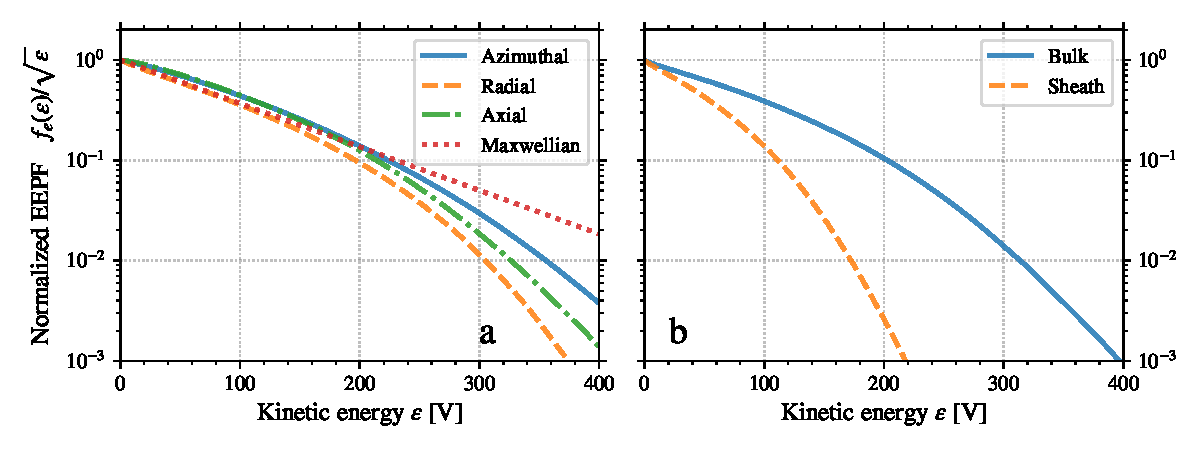
\includegraphics[width=\textwidth]{EEDF_2.pdf}
       \caption{Electron energy distribution function of the electrons ({\bf a}) in the bulk, in the three directions, and ({\bf b}) in the bulk and in the sheath. In ({\bf a}) is overlaid a Maxwellian distribution of $\Te=50\,\volt$. }
       \label{fig-EEDF}
     \end{figure}
     
    We see in \cref{fig-EEDF}.{\bf a} that the electron distribution function is not Maxwellian.
    In particular the high energy tails are depleted.
    In order to evaluate the effect of the non Maxwellian EEPF, we numerically integrate the EEPF from the PIC data using \cref{eq-ratedifinition_evdf}.
    The results (not shown) do not differ significantly from the values of $\ratemaxw$ obtained assuming a Maxwellian distribution, using \cref{eq-seemaxw}.
    Hence, we can conclude that even if the Maxwellian hypothesis is not respected in the PIC simulations, it is not enough to explain directly the differences observed on $\rate$ in \cref{fig-seeparamesMaxw}.


    \Cref{fig-EEDF}.{\bf b} presents the EEPF for the bulk population as well as for the sheath population.
    We can see that the sheath population is colder than the population at the center, which could explain the difference of \cref{fig-seeparamesMaxw}. 
    This effect is assessed in the next section.

     Surprisingly, we do not observe in \cref{fig-EEDF} secondary electron beams in the radial  direction, unlike previous observations of \citet{sydorenko2006} with a 1D model or \citet{heron2013} with a 2D model.
     On the other hand, we do observe SEE beams when  we artificially remove the electron cyclotron drift instability by forcing Ey = 0V/m \citep{croes2017}.
     Hence, it seems that the ECDI, when simulated in 2D, quickly thermalizes the secondary electrons emitted from the walls.
     In addition, we can see in \cref{fig-EEDF}.{\bf a} that the radial EEPF is close to the EEPF in the other directions, i.e the electron are almost isotropic.
     For instance, for $\crover = 200\,\volt$  we measure $\Te_r = 41.5\,\volt$ while $\Te_{\theta} \sim \Te_z = 49\,\volt$.
     The cause of the difference with \citet{heron2013} is not yet clear, but their results were  obtained at early times when saturation of the instability has not necessarily been reached, and no electron loss in  the axial direction was accounted for.
     This is supported by \cref{fig-canon_Te_strat,fig-canon_Te_all} which show us that there is a larger anisotropy at the beginning of the simulation ($t<2\micro\second$) than later.
     It is possible that at steady-state, the electrons in our simulations have had sufficient time to become more isotropic.
     The energy transfer from the axial and azimuthal directions to the radial direction is not clearly understood
     yet \citep{janhunen2018}, but we believe that it is due to the instability.



   \subsection{Radial evolution of the electron temperature}
     \label{subsec-Radial_Te}
     
     We compute the temperature in the \ac{PIC} simulations using the kinetic definition
     \[ T   = \frac{3}{2} m < (v - <v>)^2 > =  \frac{3}{2} m (<v^2> - <v>^2), \]
     with the averaging performed over the distribution function, hence
     \begin{equation} \label{eq-TeDef}
       T = \frac{3}{2} \frac{1}{n} \iiint_{\vect{v}} \norm{\vect{v} - \vect{u}}^2 f(\vect{v}) d^3v 
     \end{equation}
     with $T$ in Joule, and we have the relation with ${\rm T}$ in Volt
     \[  {\rm T} = \frac{k_b T}{e}.  \]
       
     \Cref{fig-te_profile_see} shows the radial profile of the electron temperature $\Te$ averaged in time over $5\,\micro\second$ and over the azimuthal direction, for different emissivities.
     We can see that for all of the values of $\crover$ and even without electron emission, there is a steep gradient of the electron temperature in the sheath.
     Actually, the profile of $\Te$ is very similar to the profile of the plasma potential $\phi$.
   
   \begin{figure}[hbtp]
     \centering
     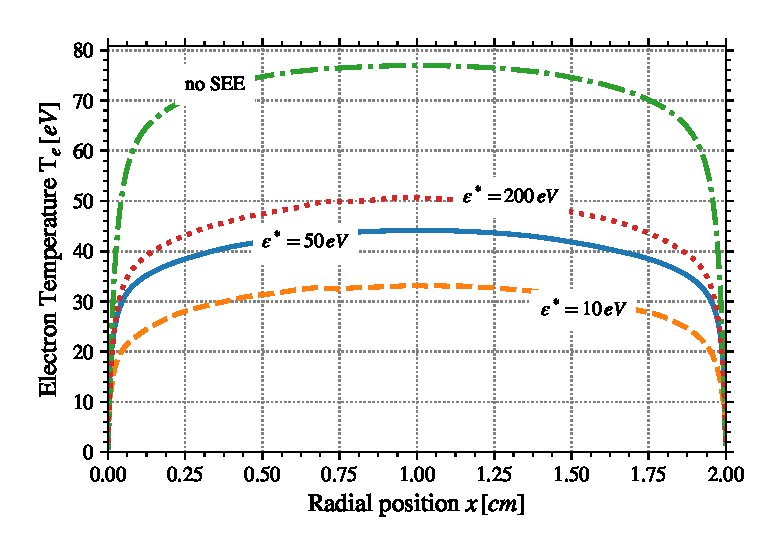
\includegraphics[width=\defaultwidth]{Te_profiles}
     \caption{Radial profiles of the electron temperature measured in the \ac{PIC} simulations, without secondary electron emission (label "no SEE") and with different values of $\crover$.}
     \label{fig-te_profile_see}
   \end{figure}
    \inlinenote{Problem with value for No SEE and \cref{fig-canon_Te_strat,fig-canon_Te_all}} 
   The significant difference between the value of the average electron temperature in the whole simulation domain, used before in \cref{sec-sheath_validation}, and the electron temperature close to the wall can be responsible of the overestimation of $\rate$ compared to $\ratepic$.
   Using this information, we compute an estimation of the electron emission rate $\rate$ with \cref{eq-seemaxw} using the electron temperature close to the wall.
   The results are presented in \Cref{fig-rate_pic_wall}.
   
   \begin{figure}[hbtp]
     \centering
     \includegraphics[width=\defaultwidth]{SEE_rates_withEEDF-eps-converted-to}
     \caption{Estimation of the electron emission rate $\rate$ as a function of $\crover$ using the values of the electron temperature close to the wall.}
     \label{fig-rate_pic_wall}
   \end{figure}
   
   We observe in \cref{fig-rate_pic_wall} that now, the electron emission rate is well predicted (error less than 5\%), except for $\crover=10\,\volt$ where a large error is still observed.
   As previously discussed, the case $\crover=10\,\volt$ presents a very high SEE rate which leads to a potential well close to the wall.
   Consequently, some secondary electrons emitted at low energy would be reflected back to the wall.
   Hence, since \cref{eq-seemaxw} does not take into account this local effect, it is not surprising that the SEE rate calculated using the mean electron temperature in the sheath is too high.
   
   To summarise, \cref{fig-rate_pic_wall} shows that when the sheath potential profile is monotonic, the \ac{SEE} rate can be well predicted by \cref{eq-seemaxw} using the electron temperature close to the wall, which is lower than in the center of the domain.
   The particle and energy flux inducing the \ac{SEE} rate are not well described if we use the electron temperature of the bulk as in the isothermal sheath model.
   This explains the overestimations of both $\rate$ and and $\dphi$ presented in \cref{fig-seeparamesMaxw,fig-Tevsproba}.
   Hence, the isothermal hypothesis used in the sheath model of \Cref{sec-sheath} is denied by the PIC simulations.
   
   In the next sections, we use a simplified \ac{PIC} simulation to study in detail the origin of the electron temperature gradient.
   

